\chapter{Kinematica van fluïda}\label{ch:b2:fluid-kinematics}

Ga op een brug staan en kijk naar de rivier. Een blad drijft voorbij,
versnelt tussen de pijlers, vertraagt in de kolk erachter, draait één keer
rond in een wervel en gaat verder. U kunt de rivier beschrijven door dat
blad te volgen --- zijn plaats en zijn snelheid op elk ogenblik --- of door
stil te blijven staan en in elk punt van de rivier op te tekenen hoe snel
het water er passeert. De tweede beschrijving is die van de fysicus: een
\emph{snelheidsveld}. Dit hoofdstuk zet de twee beschrijvingen op, leert de
versnelling van een deeltje uit het veld berekenen, schrijft het behoud van
massa als een lokale wet, en deelt stromingen in naar de vraag of zij
draaien --- de woordenschat die de vergelijkingen van Euler en Navier nodig
zullen hebben.

\begin{omfigure}
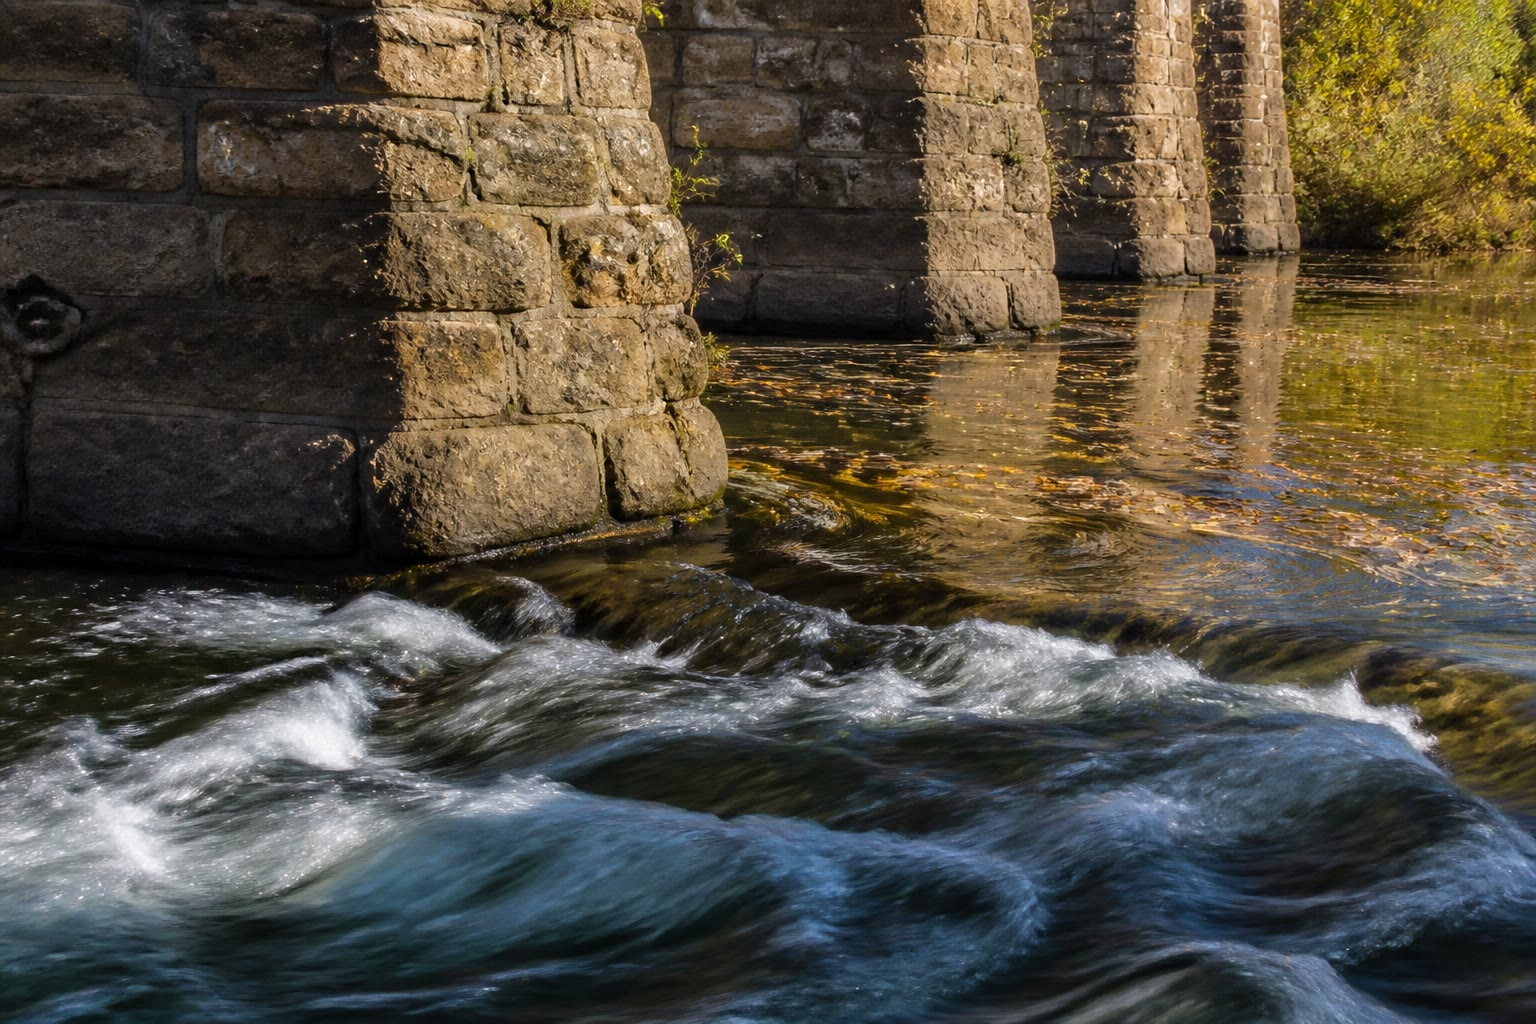
\includegraphics[width=0.58\linewidth]{images/book4/ai/b4-02-river-bridge-eddies.jpg}

{\small Een rivier voorbij een brug: snel, glad water tussen de pijlers,
wervels in hun lij --- een snelheidsveld dat men in vaste punten afleest,
geen enkele baan die men volgt.}
\end{omfigure}


\section{De continuümbeschrijving}

\begin{definition}[Fluïdumdeeltje; de continuümhypothese]\label{def:b2:fluid-kinematics:particle}
\index{fluïdumdeeltje}\index{continuümhypothese}\index{mesoscopische schaal}
Een \emph{fluïdumdeeltje} is een hoeveelheid fluïdum die klein genoeg is om
op de schaal van de stroming als een punt te gelden, en toch groot genoeg om
een enorm aantal moleculen te bevatten, zodat haar dichtheid $\rho$, druk
$P$, temperatuur $T$ en gemiddelde snelheid $\vect v$ goed gedefinieerde
gemiddelden zijn (de \emph{mesoscopische} schaal, doorgaans een micrometer).
De \emph{continuümhypothese} veronderstelt dat zo'n schaal bestaat: de
gemiddelde vrije weglengte $\ell$ van de moleculen moet veel kleiner zijn
dan de schaal $L$ van de stroming, $\ell/L \ll 1$. In lucht bij
atmosferische druk is $\ell \approx \qty{70}{nm}$; in een vloeistof is
$\ell$ de moleculaire afmeting. Het fluïdum wordt dan beschreven door
\emph{velden} $\rho(M, t)$, $P(M, t)$, $\vect v(M, t)$ die in elk punt
gedefinieerd zijn.
\end{definition}

\begin{definition}[Beschrijving van Lagrange en van Euler]\label{def:b2:fluid-kinematics:euler}
\index{beschrijving van Lagrange}\index{beschrijving van Euler}\index{stroomlijn}\index{baanlijn}\index{stationaire stroming}
De \emph{beschrijving van Lagrange} volgt elk \omterm{def:b2:fluid-kinematics:particle}{fluïdumdeeltje}: zijn plaats
$\vect r(t)$ en zijn snelheid $\dd\vect r/\dd t$ als functies van de tijd en
van zijn beginplaats. De \emph{beschrijving van Euler} geeft, in elk vast
punt $M$ en op elk tijdstip $t$, de snelheid $\vect v(M, t)$ van het deeltje
dat op dat ogenblik door $M$ komt. Een \emph{baanlijn} is de baan van een
deeltje; een \emph{stroomlijn} op het tijdstip $t$ is een kromme die in elk
punt raakt aan $\vect v(M, t)$; een \emph{stroombuis} is het oppervlak dat
de stroomlijnen door een gesloten kromme vormen. Een stroming is
\emph{stationair} wanneer de velden van Euler niet van de tijd afhangen,
$\partial\vect v/\partial t = \vect 0$; stroomlijnen en baanlijnen vallen
dan samen en liggen vast.
\end{definition}

\begin{example}[Twee beschrijvingen van één stroming]\label{ex:b2:fluid-kinematics:hose}
Water in een tuinslang met doorsnede $S$ en debiet $Q$ beweegt overal met
$v = Q/S$: het veld van Euler is uniform en de beweging van elk deeltje in
de zin van Lagrange is eenparig. In het toelopende mondstuk is het veld van
Euler nog altijd stationair, maar neemt $v$ langs de as toe: elk deeltje
\emph{versnelt} tijdens de doorgang, terwijl er in geen enkel vast punt iets
met de tijd verandert. Dat is het eerste wat de \omterm{def:b2:fluid-kinematics:euler}{beschrijving van Euler} moet
leren uitdrukken.
\end{example}

\begin{omfigure}
\begin{tikzpicture}[font=\small, x=1cm, y=1cm, >=Stealth]
  \begin{scope}
    % streamlines of a converging channel
    \foreach \y in {-1.2,-0.6,0,0.6} {
      \draw[omDef, thick, postaction={decorate, decoration={markings, mark=at position 0.55 with {\arrow{>}}}}]
        (-2.8,\y) .. controls (-0.8,\y) and (0.2,{0.45*\y}) .. (2.8,{0.45*\y});
    }
    \draw[omDef, thick, postaction={decorate, decoration={markings, mark=at position 0.55 with {\arrow{>}}}}]
        (-2.8,1.2) .. controls (-0.8,1.2) and (0.2,0.54) .. (2.8,0.54)
        coordinate[pos=0.15] (P1) coordinate[pos=0.6] (P2) coordinate[pos=0.9] (P3);
    \draw[thick] (-2.8,1.6) .. controls (-0.8,1.6) and (0.2,0.75) .. (2.8,0.75);
    \draw[thick] (-2.8,-1.6) .. controls (-0.8,-1.6) and (0.2,-0.75) .. (2.8,-0.75);
    \fill[omThm] (P1) circle (2pt) node[above, font=\footnotesize, yshift=1pt] {$t_1$};
    \fill[omThm] (P2) circle (2pt) node[above, font=\footnotesize, yshift=1pt] {$t_2$};
    \fill[omThm] (P3) circle (2pt) node[above, font=\footnotesize, yshift=1pt] {$t_3$};
    \node[font=\footnotesize, align=center] at (0,-2.15) {stationaire stroming: stroomlijnen $=$ baanlijnen,\\een deeltje versnelt waar de buis nauwer wordt};
  \end{scope}
  \begin{scope}[xshift=7.4cm]
    \draw[thick,->] (-2.8,-1.2) -- (2.8,-1.2) node[right, font=\footnotesize] {$x$};
    \draw[thick,->] (-2.8,-1.2) -- (-2.8,1.6);
    % velocity vectors at fixed points (Eulerian)
    \foreach \x in {-2.2,-1.2,-0.2,0.8,1.8} \foreach \y in {-0.6,0.2,1.0} {
      \draw[omDef, ->] (\x,\y) -- ({\x+0.5+0.12*\x},{\y+0.15*\y});
    }
    \node[omDef, font=\footnotesize] at (0,1.75) {Euler: $\vect v(M,t)$ in vaste punten};
    \draw[omThm, thick, ->] (-2.5,-0.9) .. controls (-1,-0.3) and (0.5,0.9) .. (2.4,1.3);
    \node[omThm, font=\footnotesize] at (2.2,0.7) {baanlijn};
    \node[font=\footnotesize, align=center] at (0,-1.95) {Lagrange: volg één deeltje};
  \end{scope}
\end{tikzpicture}

{\small Links: een stationaire samentrekkende stroming --- de \omterm{def:b2:fluid-kinematics:euler}{stroomlijnen}
liggen vast, een gemerkt deeltje volgt er één van en versnelt waar de buis
nauwer wordt. Rechts: de \omterm{def:b2:fluid-kinematics:euler}{beschrijving van Euler} tekent de snelheidsvector in
vaste punten op; die van Lagrange volgt een deeltje langs zijn \omterm{def:b2:fluid-kinematics:euler}{baanlijn}.}
\end{omfigure}

\section{De materiële afgeleide}

\begin{theorem}[Materiële afgeleide (deeltjesafgeleide)]\label{thm:b2:fluid-kinematics:material}
\index{materiële afgeleide}\index{convectieve versnelling}
De veranderingssnelheid van een grootheid $G(M, t)$ (scalair of vectorieel)
\emph{voor het \omterm{def:b2:fluid-kinematics:particle}{fluïdumdeeltje}} dat door $M$ komt op het tijdstip $t$, is
\[
\frac{\mathrm DG}{\mathrm Dt} = \frac{\partial G}{\partial t} + (\vect v\cdot
\operatorname{\vect{grad}})\,G ,
\qquad\text{in het bijzonder}\qquad
\vect a = \frac{\mathrm D\vect v}{\mathrm Dt} = \frac{\partial\vect v}{\partial t} +
(\vect v\cdot\operatorname{\vect{grad}})\,\vect v ,
\]
waarin
$(\vect v\cdot\operatorname{\vect{grad}}) = v_x\partial_x + v_y\partial_y +
v_z\partial_z$.
De eerste term is de \emph{lokale} veranderingssnelheid (in een vast punt),
de tweede de \emph{convectieve} (omdat het deeltje zich verplaatst naar waar
$G$ anders is). Voor de snelheid geldt
$(\vect v\cdot
\operatorname{\vect{grad}})\vect v = \operatorname{\vect{grad}}(v^2/2) +
(\operatorname{\vect{curl}}\vect v)\wedge\vect v$.
\end{theorem}

\begin{proof}
In $\dd t$ verplaatst het deeltje zich van $M$ naar $M + \vect v\,\dd t$,
zodat
$\dd G =
G(M + \vect v\dd t, t + \dd t) - G(M, t) = \partial_tG\,\dd t + \dd t\,(v_x\partial_x
+ v_y\partial_y + v_z\partial_z)G$
tot op eerste orde (kettingregel voor een functie van vier veranderlijken).
De vectoridentiteit wordt op de $x$-component nagegaan:
$[\operatorname{\vect{grad}}(v^2/2)]_x = v_x\partial_xv_x + v_y\partial_x
v_y + v_z\partial_xv_z$
en
$[(\operatorname{\vect{curl}}\vect v)\wedge\vect v]_x =
v_y(\partial_yv_x - \partial_xv_y) + v_z(\partial_zv_x - \partial_xv_z)$
(met de componenten van $\operatorname{\vect{curl}}\vect v$ zoals hieronder
gegeven in \cref{def:b2:fluid-kinematics:vorticity}); hun som is
$v_x\partial_xv_x +
v_y\partial_yv_x + v_z\partial_zv_x$.
\end{proof}

\begin{example}[Versnelling in een stationair mondstuk]\label{ex:b2:fluid-kinematics:nozzle}
Een eendimensionale \omterm{def:b2:fluid-kinematics:euler}{stationaire stroming} $v(x) = v_0(1 + x/L)$ langs een
mondstuk: de lokale term valt weg en
$a = v\,\dd v/\dd x = v_0^2(1 + x/L)/L$. Een deeltje dat binnenkomt met
$v_0 = \qty{2}{m/s}$ en met $2v_0$ vertrekt over $L
= \qty{5}{cm}$,
ondervindt $a = 80$ tot \qty{160}{m/s^2}: acht tot zestien $g$, in een
stroming waarin niets van de tijd afhangt.
\end{example}

\begin{example}[Lokaal tegenover convectief]\label{ex:b2:fluid-kinematics:weather}
De temperatuur in een weerstation daalt in de loop van de nacht
($\partial T/
\partial t < 0$: lokaal), en daalt voor een luchtpakket dat
door de wind noordwaarts wordt meegevoerd
($\vect v\cdot\operatorname{\vect{grad}}T < 0$: convectief, of
\emph{advectief}). Een thermometer aan een ballon die met de wind meedrijft,
tekent de som op, $\mathrm DT/\mathrm Dt$; het weerstation tekent alleen de
eerste term op.
\end{example}

\section{Behoud van massa}

\begin{definition}[Massadebiet en volumedebiet]\label{def:b2:fluid-kinematics:flowrate}
\index{massadebiet}\index{volumedebiet}\index{massaflux}
Het \emph{massadebiet} door een georiënteerd oppervlak $S$ is de massa die
er per tijdseenheid doorheen gaat,
$D_m = \sum\rho\,\vect v\cdot\vect n\,\dd S$ --- de flux van de
\emph{massastroomdichtheid} $\vect j = \rho\vect v$ (eenheid
\unit{kg.m^{-2}.s^{-1}}); het \emph{volumedebiet} is
$D_V = \sum\vect v
\cdot\vect n\,\dd S$ (\unit{m^3/s}). Voor een uniforme
snelheid loodrecht op een vlakke doorsnede met oppervlakte $S$ is
$D_m = \rho vS$ en $D_V = vS$.
\end{definition}

\begin{proof}
In $\dd t$ is het fluïdum dat het element $\dd S$ passeert, dat wat besloten
ligt in de scheve cilinder met grondvlak $\dd S$ en beschrijvende
$\vect v\,\dd t$, met volume $\vect v\cdot\vect n\,\dd S\,\dd t$ en massa
$\rho$ maal dat volume.
\end{proof}

\begin{theorem}[Lokaal behoud van massa]\label{thm:b2:fluid-kinematics:continuity}
\index{continuïteitsvergelijking}\index{divergentie}
In elk punt van een fluïdum geldt
\[
\frac{\partial\rho}{\partial t} + \operatorname{div}(\rho\vect v) = 0 ,
\qquad\text{waarin}\qquad
\operatorname{div}\vect A = \frac{\partial A_x}{\partial x} + \frac{\partial A_y}{\partial y} +
\frac{\partial A_z}{\partial z}
\]
de \emph{divergentie} van een vectorveld is: de netto naar buiten gerichte
flux van $\vect A$ door het oppervlak van een klein volume, per
volume-eenheid. Even goed geldt
$\mathrm D\rho/\mathrm Dt + \rho\operatorname{div}\vect v = 0$.
\end{theorem}

\begin{proof}
Neem het vaste blokje
$[x, x + \dd x]\times[y, y + \dd y]\times[z, z + \dd z]$. Zijn massa
$\rho\,\dd x\dd y\dd z$ verandert met de snelheid
$\partial_t\rho\,\dd x\dd y
\dd z$. Er komt massa binnen door het zijvlak in
$x$ met $j_x(x)\dd y\dd z$ en er gaat massa uit door het zijvlak in
$x + \dd x$ met $j_x(x + \dd x)\dd y\dd z$: netto uitstroom
$\partial_xj_x\,\dd x\dd y\dd z$, en evenzo voor $y$ en $z$. Behoud van
massa --- er wordt geen massa gemaakt --- geeft
$\partial_t\rho = -
(\partial_xj_x + \partial_yj_y + \partial_zj_z)$. De
tweede vorm volgt uit
$\operatorname{div}(\rho\vect v) = \vect v\cdot\operatorname{\vect{grad}}\rho +
\rho\operatorname{div}\vect v$.
\end{proof}

\begin{remark}[De divergentie, een eerste kennismaking]\label{rem:b2:fluid-kinematics:divergence}
De afleiding laat zien wat $\operatorname{div}$ meet: de flux die per
volume-eenheid uit een klein blokje treedt. Sommeert men over de blokjes die
een eindig volume $V$ betegelen, dan heffen de inwendige zijvlakken elkaar
paarsgewijs op en blijft alleen het buitenoppervlak over:
$\iint_{\partial V}\vect A\cdot\vect n\,\dd S = \iiint_V
\operatorname{div}\vect A\,\dd\tau$
--- de divergentiestelling (Ostrogradski), die wij netjes zullen formuleren
in \cref{ch:b2:maxwell-equations} en door de hele elektromagnetica heen
zullen gebruiken; zij wordt bewezen in het wiskundevolume van jaar 3.
Geïntegreerd over een vast volume luidt de lokale wet
$\dd m_V/\dd t = -D_m^{\text{uit}}$: de massa binnenin verandert met wat de
rand oversteekt.
\end{remark}

\begin{omfigure}
\begin{tikzpicture}[font=\small, x=1cm, y=1cm, >=Stealth]
  \begin{scope}
    \draw[thick, fill=omDef!10] (0,0) rectangle (2.2,1.6);
    \draw[thick] (0,1.6) -- (0.6,2.1) -- (2.8,2.1) -- (2.2,1.6);
    \draw[thick] (2.2,0) -- (2.8,0.5) -- (2.8,2.1);
    \draw[omThm, very thick, ->] (-1.2,0.8) -- (-0.1,0.8) node[pos=0.3, above, font=\footnotesize] {$j_x(x)$};
    \draw[omThm, very thick, ->] (2.3,0.8) -- (3.6,0.8) node[pos=0.75, above, font=\footnotesize] {$j_x(x+\dd x)$};
    \node[font=\footnotesize] at (1.1,-0.35) {$\dd x$};
    \node[font=\footnotesize] at (-0.35,0.3) {$\dd y$};
    \node[font=\footnotesize] at (2.75,-0.05) {$\dd z$};
    \node[font=\footnotesize, align=left] at (1.3,-1.1) {$\partial_t\rho\,\dd\tau = -(\partial_x j_x + \partial_y j_y + \partial_z j_z)\,\dd\tau$};
  \end{scope}
  \begin{scope}[xshift=8.2cm]
    \draw[thick] (-2.4,1.1) .. controls (-1,1.1) and (0,0.5) .. (2.4,0.5);
    \draw[thick] (-2.4,-1.1) .. controls (-1,-1.1) and (0,-0.5) .. (2.4,-0.5);
    \draw[omDef, thick] (-2.4,0) ellipse (0.25 and 1.1);
    \draw[omDef, thick] (2.4,0) ellipse (0.12 and 0.5);
    \draw[omThm, very thick, ->] (-2.4,0) -- (-1.4,0) node[above, font=\footnotesize] {$v_1$};
    \draw[omThm, very thick, ->] (2.4,0) -- (3.6,0) node[above, font=\footnotesize] {$v_2$};
    \node[omDef, font=\footnotesize] at (-2.4,1.45) {$S_1$};
    \node[omDef, font=\footnotesize] at (2.4,0.85) {$S_2$};
    \node[font=\footnotesize] at (0,-1.6) {stationair: $\rho_1v_1S_1 = \rho_2v_2S_2$};
  \end{scope}
\end{tikzpicture}

{\small Links: de massabalans van een vast blokje --- de netto uitstroom
door zijn zes zijvlakken, per volume-eenheid, is de divergentie van
$\rho\vect v$. Rechts: in een \omterm{def:b2:fluid-kinematics:euler}{stationaire stroming} is het \omterm{def:b2:fluid-kinematics:flowrate}{massadebiet} door
elke doorsnede van een stroombuis hetzelfde.}
\end{omfigure}

\begin{corollary}[Onsamendrukbare stroming; stroombuizen]\label{cor:b2:fluid-kinematics:incompressible}
\index{onsamendrukbare stroming}
Een stroming heet \emph{onsamendrukbaar} wanneer de dichtheid van elk
deeltje constant blijft, $\mathrm D\rho/\mathrm Dt = 0$, wat gelijkwaardig
is met
\[
\operatorname{div}\vect v = 0 .
\]
Een homogene vloeistof stroomt onsamendrukbaar; een gas ook, zolang de
snelheden ver onder de geluidssnelheid blijven (zie
\cref{ch:b2:sound-waves}). In een \omterm{def:b2:fluid-kinematics:euler}{stationaire stroming} is het \omterm{def:b2:fluid-kinematics:flowrate}{massadebiet}
$\rho vS$ door elke doorsnede van een stroombuis hetzelfde; is de stroming
bovendien onsamendrukbaar en $\rho$ uniform, dan is $vS$ constant: het
fluïdum versnelt waar de buis nauwer wordt.
\end{corollary}

\begin{proof}
$\mathrm D\rho/\mathrm Dt = -\rho\operatorname{div}\vect v$. Voor de buis
past men de geïntegreerde balans toe op het volume tussen twee doorsneden:
geen flux door het zijoppervlak (de snelheid raakt eraan), stationaire
toestand, dus instroom gelijk aan uitstroom.
\end{proof}

\begin{example}[Bloed]\label{ex:b2:fluid-kinematics:blood}
De aorta (doorsnede \qty{2.5}{cm^2}) voert \qty{5}{L/min}
$= \qty{83}{cm^3/s}$: $v = \qty{33}{cm/s}$. Datzelfde debiet gaat door
ongeveer $10^{10}$ haarvaten met een totale doorsnede van zo'n
\qty{2500}{cm^2}: $v = \qty{0.3}{mm/s}$ --- traag genoeg voor uitwisseling
door de wanden, wat het doel van de vertakking is.
\end{example}

\section{Vorticiteit en rotatievrije stromingen}

\begin{definition}[Vorticiteit]\label{def:b2:fluid-kinematics:vorticity}
\index{vorticiteit}\index{rotatie (van een vectorveld)}\index{rotatievrije stroming}
De \emph{vorticiteit} van een stroming is het vectorveld
\[
\vect\omega = \operatorname{\vect{curl}}\vect v , \qquad
\operatorname{\vect{curl}}\vect A = \Bigl(\frac{\partial A_z}{\partial y} -
\frac{\partial A_y}{\partial z},\; \frac{\partial A_x}{\partial z} - \frac{\partial A_z}
{\partial x},\; \frac{\partial A_y}{\partial x} - \frac{\partial A_x}{\partial y}\Bigr) .
\]
Een stroming is \emph{rotatievrij} waar $\vect\omega = \vect 0$.
\end{definition}

\begin{proposition}[Vorticiteit meet de lokale rotatie]\label{prop:b2:fluid-kinematics:rotation}
Een klein fluïdumelement met middelpunt $M$ draait, als geheel, met de
hoeksnelheid $\vect\Omega = \tfrac12\vect\omega(M)$. In een rotatie als \omterm{def:b2:rigid-body-mechanics:solid}{star
lichaam}, $\vect v = \vect\Omega\wedge\vect{OM}$, is de \omterm{def:b2:fluid-kinematics:vorticity}{vorticiteit} uniform,
$\vect\omega = 2\vect\Omega$; in de vlakke afschuifstroming
$\vect v = ky\,\vect e_x$ is zij $\vect\omega = -k\vect e_z$: een
schoepenradje dat men in een afschuifstroming laat vallen, draait rond
hoewel de \omterm{def:b2:fluid-kinematics:euler}{stroomlijnen} recht zijn.
\end{proposition}

\begin{proof}
Nabij $M$ is
$\vect v(M + \vect\epsilon) = \vect v(M) + \mathbf G\vect\epsilon$ met
$\mathbf G$ de matrix van $\partial_jv_i$; splits haar in haar symmetrische
deel (een zuivere vervorming, die het element rekt zonder het als geheel te
draaien) en haar antisymmetrische deel, waarvan de matrix
$\tfrac12(\partial_jv_i -
\partial_iv_j)$ die van
$\vect\epsilon \mapsto \tfrac12\vect\omega\wedge\vect\epsilon$ is
(\cref{thm:b2:rigid-body-mechanics:field}). Rotatie als \omterm{def:b2:rigid-body-mechanics:solid}{star lichaam} om
$\vect e_z$: $\vect v = \Omega(-y, x, 0)$,
$\omega_z = \partial_xv_y - \partial_yv_x = 2\Omega$. Afschuiving:
$\omega_z = -\partial_y(ky) = -k$.
\end{proof}

\begin{definition}[Snelheidspotentiaal; circulatie]\label{def:b2:fluid-kinematics:potential}
\index{snelheidspotentiaal}\index{circulatie (van de snelheid)}\index{potentiaalstroming}
In een \omterm{def:b2:fluid-kinematics:vorticity}{rotatievrije stroming} is de snelheid afgeleid van een
\emph{snelheidspotentiaal}: $\vect v = \operatorname{\vect{grad}}\varphi$
(de circulatie van $\vect v$ langs een weg hangt dan alleen van de uiteinden
af, $\int_A^B\vect v
\cdot\dd\vect l = \varphi(B) - \varphi(A)$). Is de
stroming bovendien onsamendrukbaar, dan is
$\Delta\varphi = \operatorname{div}\operatorname{\vect{grad}}
\varphi = 0$:
de potentiaal voldoet aan de vergelijking van Laplace, net als de
elektrostatische potentiaal in een ladingsvrij gebied --- een
\emph{potentiaalstroming}. De \emph{circulatie} van de snelheid langs een
gesloten kromme $C$ is $\Gamma = \oint_C\vect v\cdot\dd\vect l$.
\end{definition}

\begin{proof}
Dat een rotatievrij veld op een enkelvoudig samenhangend gebied een gradiënt
is, en dat een gradiënt rotatievrij is
($\partial_y\partial_z\varphi = \partial_z\partial_y\varphi$), hoort bij het
wiskundevolume van jaar 2; de vergelijking van Laplace volgt uit
$\operatorname{div}\vect v = 0$.
\end{proof}

\begin{example}[Drie vlakke stromingen]\label{ex:b2:fluid-kinematics:planeflows}
\index{stuwpuntstroming}\index{puntwervel}\index{wervel van Rankine}
(i) \emph{Stuwpuntstroming} $\vect v = k(x, -y)$:
$\operatorname{div}\vect v =
0$, $\vect\omega = \vect 0$,
$\varphi = \tfrac12k(x^2 - y^2)$; \omterm{def:b2:fluid-kinematics:euler}{stroomlijnen} $xy = $ const, hyperbolen ---
een straal die een wand treft, dicht bij de as. (ii) \emph{\omterm{ex:b2:fluid-kinematics:planeflows}{Puntwervel}}
$\vect v = \dfrac{\Gamma}{2\pi r}\vect e_\theta$ (vlakke poolcoördinaten):
onsamendrukbaar en \emph{overal rotatievrij behalve in $r = 0$},
$\varphi = \Gamma\theta/2\pi$ (meerwaardig), en de circulatie op elke cirkel
om het middelpunt is $\Gamma$ --- de \omterm{def:b2:fluid-kinematics:vorticity}{vorticiteit} zit geconcentreerd op de
as. (iii) \emph{\omterm{ex:b2:fluid-kinematics:planeflows}{Wervel van Rankine}}: een kern $r < a$ die als \omterm{def:b2:rigid-body-mechanics:solid}{star lichaam}
draait, $v_\theta = \Omega r$ (\omterm{def:b2:fluid-kinematics:vorticity}{vorticiteit} $2\Omega$), aangesloten op de
\omterm{ex:b2:fluid-kinematics:planeflows}{puntwervel} $v_\theta = \Omega a^2/r$ daarbuiten: het model van een tornado,
van een draaikolk in het bad of van de wervel achter de brugpijler --- de
snelheid is maximaal aan de rand van de kern.
\end{example}

\begin{omfigure}
\begin{tikzpicture}[font=\small, x=1cm, y=1cm, >=Stealth]
  \begin{scope}
    \foreach \c in {0.3,0.8,1.6,2.8} {
      \draw[omDef, thick, domain={\c/2.4}:2.4, samples=40, postaction={decorate, decoration={markings, mark=at position 0.5 with {\arrow{>}}}}] plot (\x,{\c/\x});
      \draw[omDef, thick, domain=-2.4:{-\c/2.4}, samples=40, postaction={decorate, decoration={markings, mark=at position 0.5 with {\arrow{<}}}}] plot (\x,{-\c/\x});
    }
    \draw[thick] (-2.5,0) -- (2.5,0);
    \draw[->] (0,0) -- (0,2.6) node[right, font=\footnotesize] {$y$};
    \node[font=\footnotesize] at (0,-0.4) {stuwpuntstroming $\vect v = k(x,-y)$};
  \end{scope}
  \begin{scope}[xshift=6.6cm]
    \foreach \r in {0.5,0.9,1.3,1.7} \draw[omDef, thick, postaction={decorate, decoration={markings, mark=at position 0.25 with {\arrow{>}}}}] (0,0) circle (\r);
    \fill (0,0) circle (1.5pt);
    \node[font=\footnotesize] at (0,-2.2) {puntwervel $v_\theta = \Gamma/2\pi r$};
  \end{scope}
  \begin{scope}[xshift=10.6cm]
    \begin{axis}[omaxis, axis x line=bottom, axis y line=left, width=4.4cm, height=3.9cm, at={(0,-1.9cm)},
        xlabel={$r/a$}, ylabel={$v_\theta$}, xmin=0, xmax=4, ymin=0, ymax=1.2, xtick={1,2,3}, ytick=\empty,
        xlabel style={at={(axis description cs:0.5,-0.12)}, anchor=north},
        ylabel style={at={(axis description cs:-0.08,0.5)}, rotate=90, anchor=south}, samples=60]
      \addplot[omThm, thick, domain=0:1] {x};
      \addplot[omThm, thick, domain=1:4] {1/x};
      \node[font=\scriptsize] at (axis cs:0.55,0.85) {$\Omega r$};
      \node[font=\scriptsize] at (axis cs:2.6,0.62) {$\Omega a^2/r$};
    \end{axis}
  \end{scope}
\end{tikzpicture}

{\small Drie vlakke stromingen. Links: de stuwpuntstroming, rotatievrij, met
hyperbolische \omterm{def:b2:fluid-kinematics:euler}{stroomlijnen}. Midden: de \omterm{ex:b2:fluid-kinematics:planeflows}{puntwervel} --- cirkelvormige
\omterm{def:b2:fluid-kinematics:euler}{stroomlijnen}, en toch \omterm{def:b2:fluid-kinematics:vorticity}{vorticiteit} nul buiten het middelpunt. Rechts: het
profiel van de \omterm{ex:b2:fluid-kinematics:planeflows}{wervel van Rankine}, rotatie als \omterm{def:b2:rigid-body-mechanics:solid}{star lichaam} in de kern en
een \omterm{ex:b2:fluid-kinematics:planeflows}{puntwervel} daarbuiten.}
\end{omfigure}

\begin{remark}[Waarom de circulatie ertoe doet]\label{rem:b2:fluid-kinematics:stokes}
Voor een kleine vlakke lus met oppervlakte $\dd S$ en normaal $\vect n$ is
de circulatie $\oint\vect v\cdot\dd\vect l = \vect\omega\cdot\vect n\,\dd S$
--- de \omterm{def:b2:fluid-kinematics:vorticity}{vorticiteit} is de circulatie per oppervlakte-eenheid, precies zoals
de divergentie de flux per volume-eenheid is. (Ga het na op de rotatie als
\omterm{def:b2:rigid-body-mechanics:solid}{star lichaam}: $2\pi r\cdot\Omega r = 2\Omega\cdot\pi r^2$.) Gesommeerd over
een oppervlak geeft dit de stelling van Stokes,
$\oint_C\vect v\cdot\dd\vect l = \iint_S
\operatorname{\vect{curl}}\vect v\cdot\vect n\,\dd S$,
geformuleerd in \cref{ch:b2:maxwell-equations}. Een vleugel wekt draagkracht
op door een circulatie om zich heen te dragen; een wervellijn blijft in een
volmaakt fluïdum bestaan (stelling van Kelvin) --- en daarom houdt de wervel
achter de pijler het zo lang uit.
\end{remark}

\begin{method}[Een snelheidsveld lezen]\label{met:b2:fluid-kinematics:reading}
Gegeven $\vect v(M, t)$: (1) is zij stationair?
($\partial_t\vect v = \vect 0$); (2) is zij onsamendrukbaar?
($\operatorname{div}\vect v = 0$); (3) is zij rotatievrij?
($\operatorname{\vect{curl}}\vect v = \vect 0$; zo ja, bepaal $\varphi$);
(4) bepaal de \omterm{def:b2:fluid-kinematics:euler}{stroomlijnen} uit $\dd x/v_x = \dd y/v_y = \dd z/
v_z$ bij
vaste $t$, en de \omterm{def:b2:fluid-kinematics:euler}{baanlijnen} uit $\dd\vect r/\dd t = \vect v(\vect r,
t)$;
(5) bereken de versnelling
$\partial_t\vect v + (\vect v\cdot
\operatorname{\vect{grad}})\vect v$. In
vlakke poolcoördinaten $(r, \theta)$ is
$\operatorname{div}\vect v = \dfrac1r\dfrac{\partial(rv_r)}{\partial r} + \dfrac1r
\dfrac{\partial v_\theta}{\partial\theta}$
en
$\omega_z = \dfrac1r\dfrac{\partial(rv_\theta)}
{\partial r} - \dfrac1r\dfrac{\partial v_r}{\partial\theta}$
(hier aangenomen; afgeleid in \cref{ch:b2:maxwell-equations}).
\end{method}

\section{Oefeningen}

\begin{exercise}[$\star$]\label{exo:b2:fluid-kinematics:1}
De gemiddelde vrije weglengte in lucht is \qty{70}{nm} bij \qty{1}{bar} en
verandert als $1/P$. Geldt de continuümbeschrijving voor (a) lucht rond een
auto, (b) lucht in een microkanaal van \qty{1}{\micro m} bij \qty{1}{bar},
(c) lucht op \qty{100}{km} hoogte ($P \approx \qty{3e-7}{bar}$) rond een
satelliet van \qty{1}{m}? Geef in elk geval $\ell/L$.
\end{exercise}

\begin{exercise}[$\star$]\label{exo:b2:fluid-kinematics:2}
Stationaire eendimensionale stroming $v(x) = v_0(1 + x/L)$ voor
$0 \le x \le L$. Versnelling van een deeltje in $x$; tijd die het nodig
heeft om van $0$ tot $L$ te komen; vergelijk met $L/v_0$ en $L/2v_0$.
\end{exercise}

\begin{exercise}[$\star$]\label{exo:b2:fluid-kinematics:3}
In een buis met straal $R$ is het snelheidsprofiel langs de as
$v(r) = v_{\max}(1 -
r^2/R^2)$. \omterm{def:b2:fluid-kinematics:flowrate}{Volumedebiet}; gemiddelde snelheid
$\langle v\rangle
= D_V/\pi R^2$; getallen voor $R = \qty{5}{mm}$,
$v_{\max} = \qty{0.4}{m/s}$.
\end{exercise}

\begin{exercise}[$\star$]\label{exo:b2:fluid-kinematics:4}
Zeg voor elk veld of de stroming onsamendrukbaar is en of zij rotatievrij
is; geef de \omterm{def:b2:fluid-kinematics:vorticity}{vorticiteit}: (a) $\vect v = (ax, -ay, 0)$; (b)
$\vect v = (-\Omega y, \Omega x, 0)$; (c) $\vect v = (ax, ay, 0)$; (d)
$\vect v =
(ky, 0, 0)$; (e) $\vect v = (ax, -ay, bz)$ --- voor welke $b$ is
zij onsamendrukbaar?
\end{exercise}

\begin{exercise}[$\star\star$]\label{exo:b2:fluid-kinematics:5}
Een tuinslang met inwendige diameter \qty{12}{mm} vult een emmer van
\qty{10}{L} in \qty{50}{s}. Snelheid in de slang; snelheid in een mondstuk
van \qty{3}{mm}; loopt het mondstuk over \qty{4}{cm} toe, schat dan de
gemiddelde versnelling van een deeltje dat het doorloopt (in $g$); tijd die
het in het mondstuk doorbrengt.
\end{exercise}

\begin{exercise}[$\star\star$]\label{exo:b2:fluid-kinematics:6}
Niet-stationaire vlakke stroming $\vect v = (U, V\cos\omega t)$ met $U$,
$V$, $\omega$ constant. (a) \omterm{def:b2:fluid-kinematics:euler}{Stroomlijnen} op het tijdstip $t$. (b) \omterm{def:b2:fluid-kinematics:euler}{Baanlijn}
van het deeltje dat op $t = 0$ in de oorsprong is. (c) Schets beide voor
$V = U$ op $t = 0$ en op $t = \pi/2\omega$; waarom verschillen zij? (d)
Versnelling van een deeltje.
\end{exercise}

\begin{exercise}[$\star\star$]\label{exo:b2:fluid-kinematics:7}
Een rivier van \qty{50}{m} breed en \qty{2.0}{m} diep stroomt met
\qty{1.2}{m/s}. (a) Debiet. (b) Zij komt een kloof binnen van \qty{15}{m}
breed en \qty{4.0}{m} diep: snelheid. (c) Een zijrivier voegt
\qty{30}{m^3/s} toe; stroomafwaarts is de rivier \qty{60}{m} breed en
\qty{2.5}{m} diep: snelheid. (d) Heet gas stroomt stationair door een buis
met constante doorsnede; tussen twee punten verdubbelt zijn temperatuur bij
constante druk: wat gebeurt er met zijn snelheid?
\end{exercise}

\begin{exercise}[$\star\star$]\label{exo:b2:fluid-kinematics:8}
\emph{\omterm{ex:b2:fluid-kinematics:planeflows}{Wervel van Rankine}.} $v_\theta = \Omega r$ voor $r < a$,
$v_\theta = \Omega a^2/r$ voor $r > a$. (a) \omterm{def:b2:fluid-kinematics:vorticity}{Vorticiteit} in elk gebied
(gebruik de formule in poolcoördinaten). (b) Circulatie op een cirkel met
straal $r$ om de as, in beide gebieden; breng die in verband met de
vorticiteitsflux. (c) Een tornado: $a = \qty{50}{m}$,
$v_{\max} = \qty{70}{m/s}$: $\Omega$, $\Gamma$, en de snelheid op
\qty{500}{m}. (d) Is de stroming in de kern rotatievrij? En daarbuiten? Waar
zit de ``rotatie'' fysisch?
\end{exercise}

\begin{exercise}[$\star\star$]\label{exo:b2:fluid-kinematics:9}
\emph{Stuwpuntstroming} $\vect v = k(x, -y)$. (a) Potentiaal $\varphi$ en ga
na dat $\Delta\varphi = 0$. (b) \omterm{def:b2:fluid-kinematics:euler}{Stroomlijnen}; de functie $\psi = kxy$ is er
constant op --- toon aan dat $v_x = \partial\psi/\partial y$,
$v_y = -\partial\psi/
\partial x$ (de \emph{stroomfunctie}). (c)
Versnellingsveld; toon aan dat het $\operatorname{\vect{grad}}(v^2/2)$ is,
en duid dat. (d) \omterm{def:b2:fluid-kinematics:euler}{Baanlijn} van een deeltje dat in $(x_0, y_0)$ vertrekt:
$x = x_0\eu^{kt}$, $y = y_0\eu^{-kt}$.
\end{exercise}

\begin{exercise}[$\star\star\star$]\label{exo:b2:fluid-kinematics:10}
\emph{Een uitdijende stroming.} Eendimensionale stroming
$v(x, t) = x/(t + \tau)$ voor $t > 0$, met $\tau > 0$ constant. (a)
\omterm{def:b2:fluid-kinematics:euler}{Baanlijnen}: toon aan dat $x(t) = x_0(1 +
t/\tau)$; versnelling van een
deeltje, zowel uit de \omterm{def:b2:fluid-kinematics:euler}{baanlijn} als uit de \omterm{thm:b2:fluid-kinematics:material}{materiële afgeleide}. (b) De
dichtheid is op elk tijdstip uniform, $\rho(t)$: bepaal $\rho(t)$ met behoud
van massa. (c) Controleer dat door de massa tussen twee deeltjes te volgen.
(d) Waarom is dit veld een eendimensionaal model van een uniform uitdijend
heelal?
\end{exercise}

\begin{exercise}[$\star\star\star$]\label{exo:b2:fluid-kinematics:11}
\emph{Bron in een stroom.} Superponeer een uniforme stroming
$\vect v = U\vect e_x$ en een vlakke bron
$\vect v = \dfrac{q}{2\pi r}\vect e_r$ ($q$ het \omterm{def:b2:fluid-kinematics:flowrate}{volumedebiet} per
lengte-eenheid langs $z$). (a) Potentiaal $\varphi = Ux +
(q/2\pi)\ln r$; ga
na dat beide stromingen onsamendrukbaar en rotatievrij zijn (behalve in de
oorsprong). (b) Stuwpunt. (c) Stroomfunctie $\psi
= Uy + q\theta/2\pi$; de
\omterm{def:b2:fluid-kinematics:euler}{stroomlijn} door het stuwpunt is $r\sin\theta = (q/2\pi U)(\pi - \theta)$:
schets haar. (d) Toon aan dat deze \omterm{def:b2:fluid-kinematics:euler}{stroomlijn} ver stroomafwaarts op
$y = \pm q/2U$ ligt: de stroming erbuiten is de stroming om een stomp
halflichaam met breedte $q/U$.
\end{exercise}

\begin{exercise}[$\star\star\star$]\label{exo:b2:fluid-kinematics:12}
\emph{Wervel en put.} Vlakke stroming
$\vect v = -\dfrac{q}{2\pi r}\vect e_r +
\dfrac{\Gamma}{2\pi r}\vect e_\theta$
voor $r > a$. (a) Toon aan dat zij onsamendrukbaar en rotatievrij is. (b)
\omterm{def:b2:fluid-kinematics:euler}{Stroomlijnen}: logaritmische spiralen $r = r_0\eu^{-q\theta/\Gamma}$. (c)
Versnelling van een deeltje: toon aan dat zij zuiver radiaal is,
$-v^2/r\,\vect e_r$. (d) Tijd waarin een deeltje van $r_0$ naar $a$
spiraliseert; aantal omwentelingen dat het daarbij maakt. (e) Getallen:
$q =
\qty{1.5e-3}{m^2/s}$, $\Gamma = \qty{3e-2}{m^2/s}$,
$r_0 = \qty{0.5}{m}$, $a = \qty{2}{cm}$.
\end{exercise}

\section{Vraagstuk: Van het afvoerputje tot de orkaan}

\begin{problem}[{Weekendvraagstuk --- dezelfde kinematica op drie schalen:
de draaikolk boven een afvoer, een tornado, en een cycloon vanuit een
satelliet gezien}]
\label{pb:b2:fluid-kinematics:1}

\medskip
\noindent\textbf{Deel I --- Het bad.}
Een bad loopt leeg door een gat met straal $a = \qty{2}{cm}$; het water, met
diepte $h = \qty{20}{cm}$, vertrekt met het \omterm{def:b2:fluid-kinematics:flowrate}{volumedebiet}
$D_V =
\qty{0.30}{L/s}$. Weg van het gat wordt de stroming als vlak
gemodelleerd (onafhankelijk van de diepte):
$\vect v = v_r(r)\vect e_r + v_\theta(r)\vect e_\theta$.
\begin{enumerate}
  \item Toon met behoud van massa door een cilinder met straal $r$ en hoogte
        $h$ aan dat $v_r = -q/2\pi r$ met $q = D_V/h$; waarde van $q$.
  \item Voordat de stop eruit ging, was het water geroerd en draaide het met
        \qty{1.0}{cm/s} op $r = \qty{50}{cm}$. Aannemend dat elke waterring
        zijn impulsmoment behoudt terwijl hij naar binnen trekt ($rv_\theta$
        constant), bepaal $v_\theta(r)$ en de circulatie $\Gamma$.
  \item Ga na dat de stroming onsamendrukbaar en rotatievrij is voor $r > a$.
  \item \omterm{def:b2:fluid-kinematics:euler}{Stroomlijnen}: toon aan dat het logaritmische spiralen zijn en bepaal
        hoeveel omwentelingen een deeltje maakt tussen $r = \qty{50}{cm}$ en
        $r = a$.
  \item Tijd waarin een deeltje van \qty{50}{cm} tot het gat gaat, en zijn
        azimutale snelheid bij aankomst.
  \item Versnelling van een deeltje in $r$; vergelijk met $g$ voor $r = a$.
        (Het vrije oppervlak zakt in waar de druk daarmee in evenwicht moet
        zijn --- de trechter; volgend hoofdstuk.)
  \item De draaiing van de aarde geeft elk fluïdum dat in het bad in rust is
        een ``achtergrondrotatie'' met de plaatselijke verticale snelheid
        $\Omega_\oplus\sin\lambda \approx \qty{5e-5}{rad/s}$. Vergelijk de
        azimutale snelheid die zij op \qty{50}{cm} zou geven met de
        \qty{1}{cm/s} van het roeren, en zeg of het halfrond de
        draairichting van een leeglopend bad bepaalt.
\end{enumerate}

\medskip
\noindent\textbf{Deel II --- De tornado als \omterm{ex:b2:fluid-kinematics:planeflows}{wervel van Rankine}.}
Kernstraal $a = \qty{60}{m}$, maximale wind $v_{\max} = \qty{80}{m/s}$,
luchtdichtheid $\rho = \qty{1.2}{kg/m^3}$.
\begin{enumerate}[resume]
  \item Schrijf $v_\theta(r)$ in beide gebieden op en geef $\Omega$ en $\Gamma$.
  \item \omterm{def:b2:fluid-kinematics:vorticity}{Vorticiteit} in de kern en daarbuiten; schets $v_\theta$ en
        $\omega_z$ tegen $r$.
  \item Versnelling van een luchtdeeltje aan de rand van de kern; vergelijk met $g$.
  \item Toon aan dat een klein schoepenrad buiten de kern om de tornado heen
        drijft zonder om zijn eigen as te draaien, terwijl een schoepenrad
        in de kern één keer per omloop om de as draait.
  \item Kinetische energie van de kern, per meter hoogte.
  \item Kinetische energie van de stroming daarbuiten per meter hoogte,
        tussen $a$ en $R = \qty{5}{km}$; waarom hangt zij alleen
        logaritmisch van $R$ af?
  \item Totale kinetische energie bij een hoogte van \qty{1}{km}; vergelijk
        met de energie die \qty{1}{t} TNT vrijmaakt (\qty{4.2}{GJ}).
  \item In een tornado stroomt de lucht ook naar binnen en naar boven. Wordt
        de kern over de eerste \qty{300}{m} hoogte door een radiale instroom
        van \qty{5}{m/s} door haar zijoppervlak gevoed, welke verticale
        snelheid moet de lucht dan boven aan die laag bereiken (uniform over
        de doorsnede van de kern)?
\end{enumerate}

\medskip
\noindent\textbf{Deel III --- De cycloon.}
Een tropische cycloon wordt gemodelleerd als een \omterm{ex:b2:fluid-kinematics:planeflows}{wervel van Rankine} met
kernstraal $a = \qty{40}{km}$ en $v_{\max} = \qty{50}{m/s}$. De draaiing van
de aarde laat zich voelen via de \emph{planetaire \omterm{def:b2:fluid-kinematics:vorticity}{vorticiteit}}
$f = 2\Omega_\oplus\sin\lambda
\approx \qty{5e-5}{s^{-1}}$ op breedtegraad
\qty{20}{\degree}: een luchtring die ten opzichte van de grond in rust is,
draagt in het inertiaalstelsel al de azimutale snelheid $fr/2$ om elke
verticale as.
\begin{enumerate}[resume]
  \item \omterm{def:b2:fluid-kinematics:vorticity}{Vorticiteit} van de kern en circulatie $\Gamma$ van de cycloon;
        vergelijk de \omterm{def:b2:fluid-kinematics:vorticity}{vorticiteit} van de kern met $f$.
  \item Een luchtring met straal $r_0 = \qty{500}{km}$, aanvankelijk in rust
        ten opzichte van de grond, wordt door de lage druk naar het
        middelpunt getrokken. Aannemend dat zijn impulsmoment per
        massa-eenheid om de as, $r(v_\theta + fr/2)$, behouden blijft,
        bepaal zijn snelheid $v_\theta$ ten opzichte van de grond op
        $r = \qty{100}{km}$ en op $r = \qty{40}{km}$.
  \item In welke zin draait de cycloon op het noordelijk halfrond, en
        waarom? Waarom ligt die zin voor een cycloon vast en voor een bad
        niet?
  \item Waarom kan de lucht op deze manier niet helemaal tot de as worden
        getrokken --- wat begrenst de wind en laat een oog achter?
  \item De lucht convergeert met \qty{5}{m/s} naar de cycloon door een
        cilinder met straal \qty{500}{km} en hoogte \qty{1}{km}: naar binnen
        getrokken \omterm{def:b2:fluid-kinematics:flowrate}{massadebiet} ($\rho = \qty{1.2}{kg/m^3}$).
  \item De cycloon verplaatst zich als geheel westwaarts met \qty{6}{m/s}.
        Schrijf het euleriaanse snelheidsveld zoals het vanaf de grond wordt
        gezien in termen van het veld $\vect v_0$ van de wervel in haar
        eigen stelsel; is de stroming stationair in het stelsel van de
        grond? Aan welke kant van de storm waait het harder?
\end{enumerate}

\medskip
\noindent\textbf{Deel IV --- Debieten en een overzicht.}
\begin{enumerate}[resume]
  \item Er valt \qty{50}{mm/h} regen op een stroomgebied van \qty{10}{km^2}
        en alles bereikt een rivier met doorsnede \qty{40}{m^2}: gemiddelde
        snelheid van de rivier bij hoogwater.
  \item Bloed: de aorta (\qty{2.5}{cm^2}) voert \qty{5.0}{L/min}; de
        haarvaten hebben een totale doorsnede van \qty{0.25}{m^2}: snelheden
        in elk; tijd waarin bloed een haarvat van \qty{1}{mm} doorloopt.
  \item Een vat met doorsnede $S$ loopt leeg door een gat met doorsnede $s$
        in de bodem; de uitstroomsnelheid is $\sqrt{2gh}$ ($h$ het waterpeil
        --- hier aangenomen, in het volgende hoofdstuk afgeleid). Schrijf
        het behoud van massa op en bepaal $h(t)$ en de leegloop\-tijd voor
        $S = \qty{1}{m^2}$, $s = \qty{1}{cm^2}$, $h_0 = \qty{1}{m}$.
  \item Geef de drie stromingen van de delen I--III in één tabel: straal,
        snelheid, \omterm{def:b2:fluid-kinematics:vorticity}{vorticiteit} van de kern, circulatie --- en de grootheid
        die tijdens de instroom behouden blijft en hen doet opdraaien.
\end{enumerate}
\end{problem}
